%-*- mode: LaTeX; -*-
%Optical microscopy
	%Nomarski interference 
	%Reflection mode

	
\section{Nomarski interference contrast microscopy}
\label{sec:nomarski}

Nomarski interference contrast microscopy, also known as differential interference contrast microscopy, is a version of optical microscopes designed to be able to investigate the inside of samples. The method utilizes the polarization of light to give slightly different light paths depending on where in the sample the light passes. The setup is shown in figure \ref{fig:nomarski}.

\begin{figure}[h]
\begin{center}
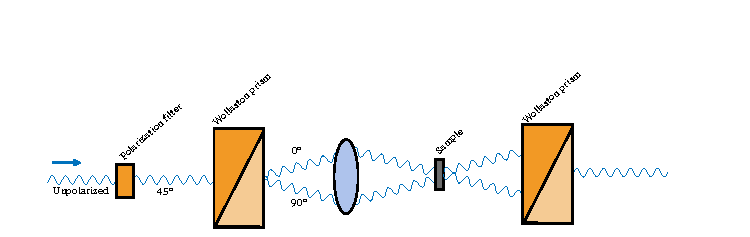
\includegraphics[scale=1]{sin.pdf}
\caption{A schematic of the Nomarski microscope setup. The light passes through the setup from the left to the right. 
\label{fig:nomarski}}
\end{center}
\end{figure}

The light is initially unpolarized. After passing a 45$^\circ$ polarization filter, the light enters a Wollaston prism. This prism will split the light in different directions depending on the polarization, creating two diverging beams. One beam will have light polarized in the 0$^\circ$ direction and the other in the $90^\circ$ direction. These two beams are focused on the sample by a lens, but made to hit the sample at slightly different positions. This will give the light beams slightly different paths through the sample. As the beams leave the sample they will enter another Wollaston prism, which will merge the two beams into one, and give the beams the same polarization, 135$^\circ$. If the beams have travelled different lengths in the sample, or if the sample composition has varied between the two paths, then the beams will be slightly out of phase. This phase difference will through interference between the beams lead to optical contrast.

One possible use for the Nomarski microscope is to detect different thickness in the sample. It can also be used to detect  sample composition difference, if the compositions have different refractive indexes. An example would be if a 3C-SiC sample has some hexagonal inclusions, then these will give contrast in the microscope since the hexagonal and cubic polytypes have slightly different refractive indexes. 






































